\section{Analysis}
\subsection{Measurement of the stability condition}
As described in Chapter~\ref{sec:theory}, in order to achieve a stable resonator
for laser emission, the stability condition~\ref{eqn:stability} must hold true.
The two mirror configurations available are Flat/Flat-Flat/$\SI{1400}{\milli\meter}$ and
Flat/$\SI{1400}{\milli\meter}$-Flat/$\SI{1400}{\milli\meter}$. The stability condition~\ref{eqn:stability}
yields a maximum resonator length of $L_{1} = r_{2} = \SI{1400}{\milli\meter}$ for the former and
$L_{2} = r_{1} + r_{2} = \SI{2800}{\milli\meter}$ for the later configuration.
To test these theoretical calculations, the achieved laser intensity in different
mirror and length configurations is measured. The resulting data is displayed in Figure~\ref{fig:distance-intensity}.
\begin{figure}[H]
 \centering
 \includegraphics[scale=0.8]{./build/Distanz-Intensität.pdf}
 \caption{Plot of the intensity measurement for different resonator configurations.}
 \label{fig:distance-intensity}
\end{figure}
\noindent
The data is given in tabular form in Table~\ref{tab:distance-intensity}.
The measurement was carried out until a consistent intensity measurement was not possible or the length of the
optical bench was reached.
\begin{table}[H]
    \centering
    \caption{Measurements of the Laser intensity for different resonator lengths and mirror configurations.}
    \label{tab:distance-intensity}
    \sisetup{table-format=3.2}
    \begin{tabular}{S S | S S}
        \toprule
        \multicolumn{2}{c|}{Flat/1400mm-Flat/1400mm} & \multicolumn{2}{c}{Flat/Flat-Flat/1400mm} \\
        {$d/\si{\centi\meter}$} & {$I/\si{\milli\watt}$} & {$d/\si{\centi\meter}$} & {$I/\si{\milli\watt}$} \\
        \midrule
        63.5 &  1.41    & 55.0 &   2.36 \\
        69.0 &  3.50    & 60.0 &   2.14 \\
        73.4 &  2.30    & 60.7 &   1.96 \\
        76.9 &  4.75    & 65.0 &   2.32 \\
        81.7 &  4.5     &  66.0 &   2.02 \\
        87.1 &  5.67    & 71.0 &   1.45 \\
        92.0 &  5.3     & 72.0 &   1.45 \\
        96.7 &  4.4     & 74.5 &   1.16 \\
        101.4 & 4.5     & 78.0 &   1.32 \\
        105.5 & 2.68    & 79.2 &   1.13 \\
        109.9 & 3.21    & 83.1 &   1.65 \\
        113.5 & 3.08    & 85.8 &   0.78 \\
        117.1 & 2.05    & 90.0 &   1.57 \\
        121.2 & 2.3     & 91.3 &   0.1 \\
        125.1 & 1.98    & 92.4 &   0 \\
        127.9 & 0.68    & 96.5 &   0 \\
        131.2 & 0.9     & 126.3 &  1.3  \\
        136.6 & 0.7     &       &       \\
        141.8 & 1.43        &       &       \\
        147.1 & 1.9     &       &       \\
        152.4 & 1.87        &       &       \\
        161.0 & 1.4     &       &       \\
        165.8 & 0.55        &       &       \\
        177.7 & 2.1     &       &       \\
        185.3 & 2.75        &       &       \\
        191.2 & 2.1     &       &       \\
        198.0 & 2.15        &       &       \\
        202.2 & 2.35        &       &       \\
        \bottomrule
    \end{tabular}
\end{table}
\noindent

\subsection{TEM Modes}
In this section, the $\text{TEM}_{00}$ and $\text{TEM}_{10}$ modes described in~\ref{sec:theory} are
observed by measuring the laser intensity perpendicular to the optical axis.
\subsubsection{\texorpdfstring{$\text{TEM}_{00}$}{TEM} Mode}
The amplitudes of the Modes are given by Equation~\eqref{eqn:TEM}. Therefore the intensity of the $\text{TEM}_{00}$ mode
is described by
\begin{equation}
 I = I_{\text{max}} \cdot \exp{\left(\frac{-{(r-r_{0})}^{2}}{2 \omega^{2}}\right)} + I_{0}.
 \label{eqn:TEM00-Fit}
\end{equation}
\noindent
Here, $I_{\text{max}}$ denotes the maximum intensity, $I_{0}$ the intensity contribution by background light, $r_{0}$ the
centre of the laser beam and $\omega$ describes the width of the gaussian curve. Measurement of the background light with the laser
being deactivated yielded an intensity of $I_{0} = \SI{0.0001}{\micro\ampere}$.
The parameters of~\eqref{eqn:TEM00-Fit} are fitted to the measurements using \texttt{scipy.optimize.curve\_fit};
the resulting values are shown below.
\begin{align*}
  I_{\text{max}} = & \SI{9.04 \pm 0.22}{\micro\ampere} \\
  r_{0} = & \SI{8.67 \pm 0.13}{\centi\meter} \\
  \omega = & \SI{4.72 \pm 0.13}{\centi\meter}.
\end{align*}
\noindent
The fitted curve and the data is displayed in Figure~\ref{fig:TEM-Messung1}.
\begin{figure}
  \centering
  \includegraphics[scale=0.8]{./build/TEM00-Mode+Pull.pdf}
  \caption{Intensity measurement of the $\text{TEM}_{00}$ mode.}
\label{fig:TEM-Messung1}
\end{figure}
\noindent
\subsubsection{\texorpdfstring{$\text{TEM}_{01}$}{TEM} Mode}
The intensity of the $\text{TEM}_{10}$ is given by equation~\eqref{eqn:TEM10-Fit}
\begin{equation}
 I = I_{\text{max}} \cdot \frac{4{(r-r_{0})}^{2}}{\omega^{2}} \cdot \exp{\bigl( \frac{-{(r-r_{0})}^{2}}{2\omega^{2}} \bigr)} + I_{0}.
 \label{eqn:TEM10-Fit}
\end{equation}
Equation~\eqref{eqn:TEM10-Fit} is again fitted to the measured data using \texttt{scipy.optimize.curve\_fit}, which yields the
parameters
\begin{align*}
  I_{\text{max}} = & \SI{0.91 \pm 0.02}{\micro\ampere} \\
  r_{0} = & \SI{6.54 \pm 0.10}{\centi\meter} \\
  \omega = & \SI{4.71 \pm 0.07}{\centi\meter}.
\end{align*}
The resulting curve is depicted in Figure~\ref{fig:TEM-Messung2}.
\begin{figure}
  \centering
  \includegraphics[scale=0.8]{./build/TEM10-Mode+Pull.pdf}
  \caption{Intensity measurement of the $\text{TEM}_{10}$ mode.}
\label{fig:TEM-Messung2}
\end{figure}
\noindent
\subsection{Polarisation of the laser}
The Brewster windows mentioned in Section~\ref{sec:procedure} ensure that most light passing through is p-polarised.
To verify this, a measurement of the intensity dependence on the polarisation angle is carried out.
The theoretical intensity curve is given by Equation~\eqref{eqn:intensity-angle}
\begin{equation}
 I = I_{\text{max}} \cdot \sin{{(\alpha + \alpha_{0})}^{2}} + I_{0},
 \label{eqn:intensity-angle}
\end{equation}
where $I_{\text{max}}$ describes the maximum intensity, $\alpha_{0}$ the zero angle and $I_{0}$ again describes the intensity
contribution by background light.
Using \texttt{scipy.optimize.curve\_fit}, this function is fitted to the measured data. The results are shown in
Figure~\ref{fig:polarisation}.
\begin{figure}
	\centering
  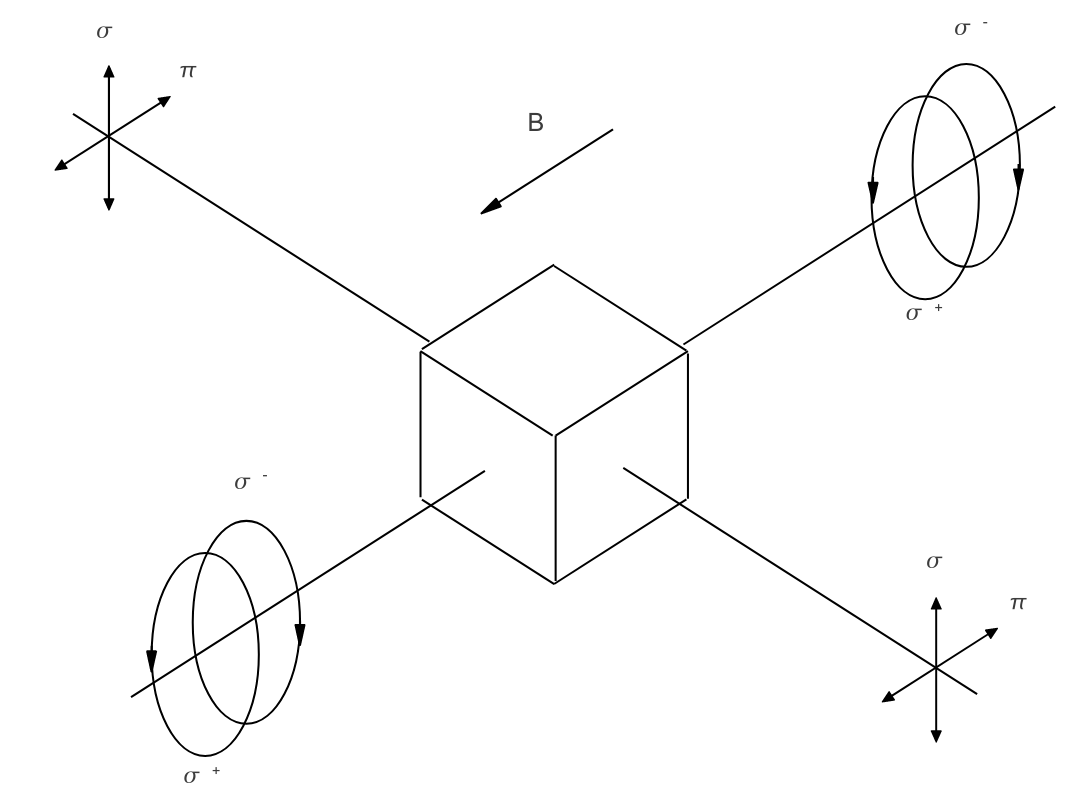
\includegraphics[scale=0.8]{./build/Polarisation.pdf}
\caption{Intensity measurement for different polarisation filter angles.}
\label{fig:polarisation}
\end{figure}
\noindent
The resulting fit parameters are
\begin{align*}
	I_{\text{max}} = \SI{2.09 \pm 0.08}{\milli\watt} \\
  I_{0} = \SI{-0.03 \pm 0.05}{\milli\watt} \\
  \alpha_{0} = \SI{194.15 \pm 1.06}{\degree}.
\end{align*}
\noindent
The measured data is given in tabulary form in Table~\ref{tab:intensity-angles}.
\begin{table}[H]
    \centering
    \caption{Measurements of the Laser intensity for different angles.}
    \label{tab:intensity-angles}
    \sisetup{table-format=3.0}
    \begin{tabular}{S S[table-format=1.2] | S S[table-format=1.2]}
        \toprule
      {$\alpha/\si{\degree}$} & {$I/\si{\milli\watt}$} & {$\alpha/\si{\degree}$} & {$I/\si{\milli\watt}$} \\
        \midrule
        0     &     0.15  & 180   &     0.13  \\
        10    &     0.39  & 190   &     0.34  \\
        20    &     0.72  & 200   &     0.66  \\
        30    &     1.13  & 210   &     0.13  \\
        40    &     1.42  & 220   &     1.41  \\
        50    &     1.75  & 230   &     1.75  \\
        60    &     1.97  & 240   &     1.96  \\
        70    &     2.05  & 250   &     2.08  \\
        80    &     2.13  & 260   &     2.12  \\
        90    &     2.00  & 270   &     1.86  \\
        100   &     1.72  & 280   &     1.68  \\
        110   &     1.46  & 290   &     1.15  \\
        120   &     1.08  & 300   &     1.04  \\
        130   &     0.67  & 310   &     0.68  \\
        140   &     0.39  & 320   &     0.37  \\
        150   &     0.14  & 330   &     0.14  \\
        160   &     0.02  & 340   &     0.02  \\
        170   &     0.02  & 350   &     0.02  \\
        \bottomrule
    \end{tabular}
\end{table}
\noindent
\subsection{Examination of the frequency spectrum of the laser}
To measure the frequency spectrum of the Helium-Neon-Laser in multi-mode operation, a fast photodiode connected to an
oscilloscope is utilized. The measurement is carried out for four different resonator lengths. The distance between the peak
frequencies is used to compare it to the theoretical mode distance given by~\eqref{eqn:modetheo}:
\begin{equation}
	\Delta f_{\text{Theory}} = \frac{c}{2\cdot L}.
  \label{eqn:modetheo}
\end{equation}
\noindent
Therefore, each mode difference has to be an integer multiple of $\Delta f_{\text{Theory}}$:
\begin{equation}
f_{\text{Theory}}	= n \cdot \Delta f_{\text{Theory}} = n \cdot \frac{c}{2 \cdot L}.
\label{eqn:modetheomultiple}
\end{equation}
\noindent
The resulting data is given in Table~\ref{tab:multimode}.
\begin{table}[H]
    \centering
    \caption{Measurements of the Laser spectrum in multi-mode operation for different resonator lengths.}
    \label{tab:multimode}
    \sisetup{table-format=4.0}
    \begin{tabular}{S[table-format=2.0] S S S S}
        \toprule
        \multicolumn{1}{c}{Peak} & \multicolumn{4}{c}{$f/\si{\mega\hertz}$} \\
        \cmidrule{2-5}
        & {$L=\SI{87.5}{\centi\meter}$} & {$L=\SI{66.8}{\centi\meter}$} & {$L=\SI{156.5}{\centi\meter}$} & {$L=\SI{215.8}{\centi\meter}$} \\
        \midrule
        1   &   188   &   255   &   105   &   221   \\
        2   &   379   &   518   &   206   &   439   \\
        3   &   570   &   773   &   308   &   653   \\
        4   &   758   &   1031  &   405   &   870   \\
        5   &   949   &         &   510   &   1084  \\
        6   &   1140  &         &   608   &   1305  \\
        7   &         &         &   709   &         \\
        8   &         &         &   814   &         \\
        9   &         &         &   911   &         \\
        10  &         &         &   1016  &         \\
        11  &         &         &   1114  &         \\
        12  &         &         &   1219  &         \\
        13  &         &         &   1320  &         \\
        \bottomrule
    \end{tabular}
\end{table}
\noindent
In Table~\ref{tab:deltaf}, the mean of the deltas between the peaks for each of the four lengths are displayed and compared
to the closest theoretical mode distance.
\begin{table}[H]
    \centering
    \caption{Comparison between the mean measured frequency deltas and the theoretical values for different resonator lengths.}
    \label{tab:deltaf}
    \sisetup{table-format=3.2}
    \begin{tabular}{S[table-format=3.1] S S S S}
        \toprule
      {$L/\si{\centi\meter}$} & {$\bar{\Delta} f/\si{\mega\hertz}$} &  {$\Delta f_{\text{Theory}}$}  & {$\bar{\Delta} f - \Delta f_{\text{Theory}}$} & {$(\bar{\Delta} f - \Delta f_{\text{Theory}}) /\si{\percent}$}\\
        \midrule
      87.5    &   190.40    &   171.3   &  19.1  & 11.15\\
      66.8    &   258.67    &   224.4   & 34.27  & 15.27\\
      156.5   &   101.25    &   95.78   & 5.47   &  5.71\\
      215.8   &   216.80    &   69.46   & 147.34 &  212.12\\
        \bottomrule
    \end{tabular}
\end{table}
\noindent
\subsection{Laser wavelength}
To determine the laser wavelength, the diffraction maxima for several different optical gratings are measured. The wavelength
can be determined by utilizing the relation~\eqref{eqn:wavelength}.
\begin{equation}
  k \lambda = d \sin{(\alpha_{k})} \Rightarrow \lambda = \frac{d \cdot a_{k}}{k \sqrt{e^{2} + a_{k}^{2}}}.
  \label{eqn:wavelength}
\end{equation}
\noindent
Here, $d$ describes the distance between the slits of the optical grating, $e$ is the distance between the optical grating and
the screen and $a_{k}$ describes the distance between the optical axis and the diffraction maximum with order $k$.
The measured values of $a_{k}$ for different optical gratings are displayed in Table~\ref{tab:opticalgr}. The first two
measurements were carried out with a distance $d=\SI{70}{\centi\meter}$ and the last two with a distance
$d=\SI{29.4}{\centi\meter}$.
\begin{table}[H]
    \centering
    \caption{Measurements of $a_{k}$ for different optical gratings.}
    \label{tab:opticalgr}
    \sisetup{table-format=3.2}
    \begin{tabular}{S S S S S}
        \toprule
      & \multicolumn{4}{c}{$a_{k}/\si{\centi\meter}$} \\
        \midrule
        {$2k$} & {$80\mathrm{l}/\si{\milli\meter}$} & {$100\mathrm{l}/\si{\milli\meter}$} & {$600\mathrm{l}/\si{\milli\meter}$} & {$1200\mathrm{l}/\si{\milli\meter}$} \\
        \midrule
        1   & 7.1   &   9.0   &   24.0    &   68.5 \\
        2   & 14.3  &   18.2  &   44.6    &        \\
        3   & 21.5  &   27.4  &           &        \\
        4   & 32.8  &   37.0  &           &        \\
        5   & 40.6  &   47.1  &           &        \\
        6   & 44.5  &   63.3  &           &        \\
        \bottomrule
    \end{tabular}
\end{table}
\noindent
The measurements in Table~\ref{tab:opticalgr} are taken from the $k$-maximum on one side of the optical axis to the $k$-maximum
on the other side of the optical axis and then halfed in the computation of $\lambda$ to reduce the uncertainty of the measurement.
The remaining measurement uncertainty is estimated to be $\sigma_{a_{k}} = \SI{0.2}{\centi\meter}$.
Using Equation~\eqref{eqn:wavelength}, the following wavelengths were obtained:
\begin{align*}
\lambda_{1} = &  \SI{422.8356 \pm 2.3245}{\nano\meter} \\
\lambda_{2} = &  \SI{664.8679 \pm 2.6663}{\nano\meter} \\
\lambda_{3} = & \SI{18548.6406 \pm 69.5400}{\nano\meter} \\
\lambda_{4} = & \SI{91054.4704 \pm 112.7858}{\nano\meter}.
\end{align*}
The average wavelength resulting of all four measurements weighted by their respective uncertainty is given by
\begin{equation}
 \bar{\lambda} = \SI{560.6150 \pm 3.5028}{\nano\meter}.
\end{equation}
